% Editable English source of the user manual.
% Compile twice from the docs directory:
%   pdflatex benutzerhandbuch-en.tex
% Requires a standard LaTeX installation with English language support.
% The corresponding German source is benutzerhandbuch-de.tex.

\documentclass[a4paper,11pt]{article}

\usepackage[T1]{fontenc}
\usepackage[utf8]{inputenc}
\usepackage[english]{babel}
\usepackage{lmodern}
\usepackage{microtype}
\usepackage[left=24mm,right=24mm,top=24mm,bottom=24mm,headheight=15pt]{geometry}
\usepackage{graphicx}
\usepackage{booktabs}
\usepackage{tabularx}
\usepackage{array}
\usepackage{fancyhdr}
\usepackage[hidelinks]{hyperref}

\hypersetup{
  pdftitle={Measure Shift -- User manual: Image alignment with the joystick},
  pdfsubject={Reference capture, pixel calibration, X alignment and incremental movement},
  pdfauthor={},
  pdflang={en}
}

\setlength{\parindent}{0pt}
\setlength{\parskip}{0.5em}
\setlength{\emergencystretch}{1.5em}
\renewcommand{\arraystretch}{1.15}
\newcolumntype{Y}{>{\raggedright\arraybackslash}X}
\newcolumntype{L}[1]{>{\raggedright\arraybackslash}p{#1}}

\pagestyle{fancy}
\fancyhf{}
\fancyhead[L]{\small Measure Shift}
\fancyhead[R]{\small User manual}
\fancyfoot[L]{\small Edition: 16 November 2026}
\fancyfoot[R]{\small Page \thepage\ of \pageref*{LastPage}}
\renewcommand{\headrulewidth}{0.4pt}
\renewcommand{\footrulewidth}{0.4pt}

% These names describe joystick functions, not button positions.
\newcommand{\ReferenceButton}{\textbf{reference button}}
\newcommand{\AlignButton}{\textbf{align button}}
\newcommand{\Status}[1]{\texttt{#1}}
\newcommand{\Note}[2]{\par\smallskip\textbf{#1}\enspace #2\par\smallskip}

\begin{document}

\begin{center}
  {\LARGE\bfseries Measure Shift\par}
  \medskip
  {\Large User manual\par}
  \smallskip
  {\large Image alignment with the joystick\par}
\end{center}

\section{Prerequisites and controls}

This manual assumes a live camera, a configured axis controller, and enabled
joystick functions. The axis controller determines the travel for each
relay press. Set the required image tolerance in the application.

\begin{tabularx}{\linewidth}{@{}L{0.28\linewidth}Y@{}}
\toprule
\textbf{Control} & \textbf{Function} \\
\midrule
Joystick left/right & Move the motor axis in steps. Holding the joystick repeats the movement. \\
\ReferenceButton & Capture the current camera image as the new reference image. \\
\AlignButton{} or \textbf{Align X} & Start direct X alignment to the current reference. \\
\textbf{Run pixel calibration} & Measure the X displacement per relay press. \\
\bottomrule
\end{tabularx}

These names refer to the functions assigned to the joystick. The exact button
positions depend on your setup.

\section{Operating procedure}

\begin{enumerate}
  \setlength{\itemsep}{0.45em}
  \item \textbf{Check readiness.} Check that the live image is updating and the
  axis is ready.

  \item \textbf{Capture a reference.} Once motion has stopped, press and release
  the \ReferenceButton{} once. The desired reference image must now appear
  on the left.

  \item \textbf{Position the part approximately.} Use the joystick to move
  the part to be aligned in steps until the feature is clearly visible in the
  image. Then release the joystick and wait for motion to stop.

  \item \textbf{Align.} Press and release the \AlignButton{} once.
  Keep the joystick in its neutral position during automatic corrections.

  \item \textbf{Check the result.} Check the axis message
  \Status{X aligned}, the X/Y values and the image overlap.
  The overall status \Status{ALIGNED} confirms that the image displacement
  is within the configured tolerance.
\end{enumerate}

\newpage
\section{Monitoring the screen}

On the left, \textbf{REFERENCE} shows the fixed reference image. On the right,
\textbf{LIVE} shows the current camera image. \textbf{Alignment} displays the
measurement status, X/Y displacement and configured tolerance.

\begin{center}
  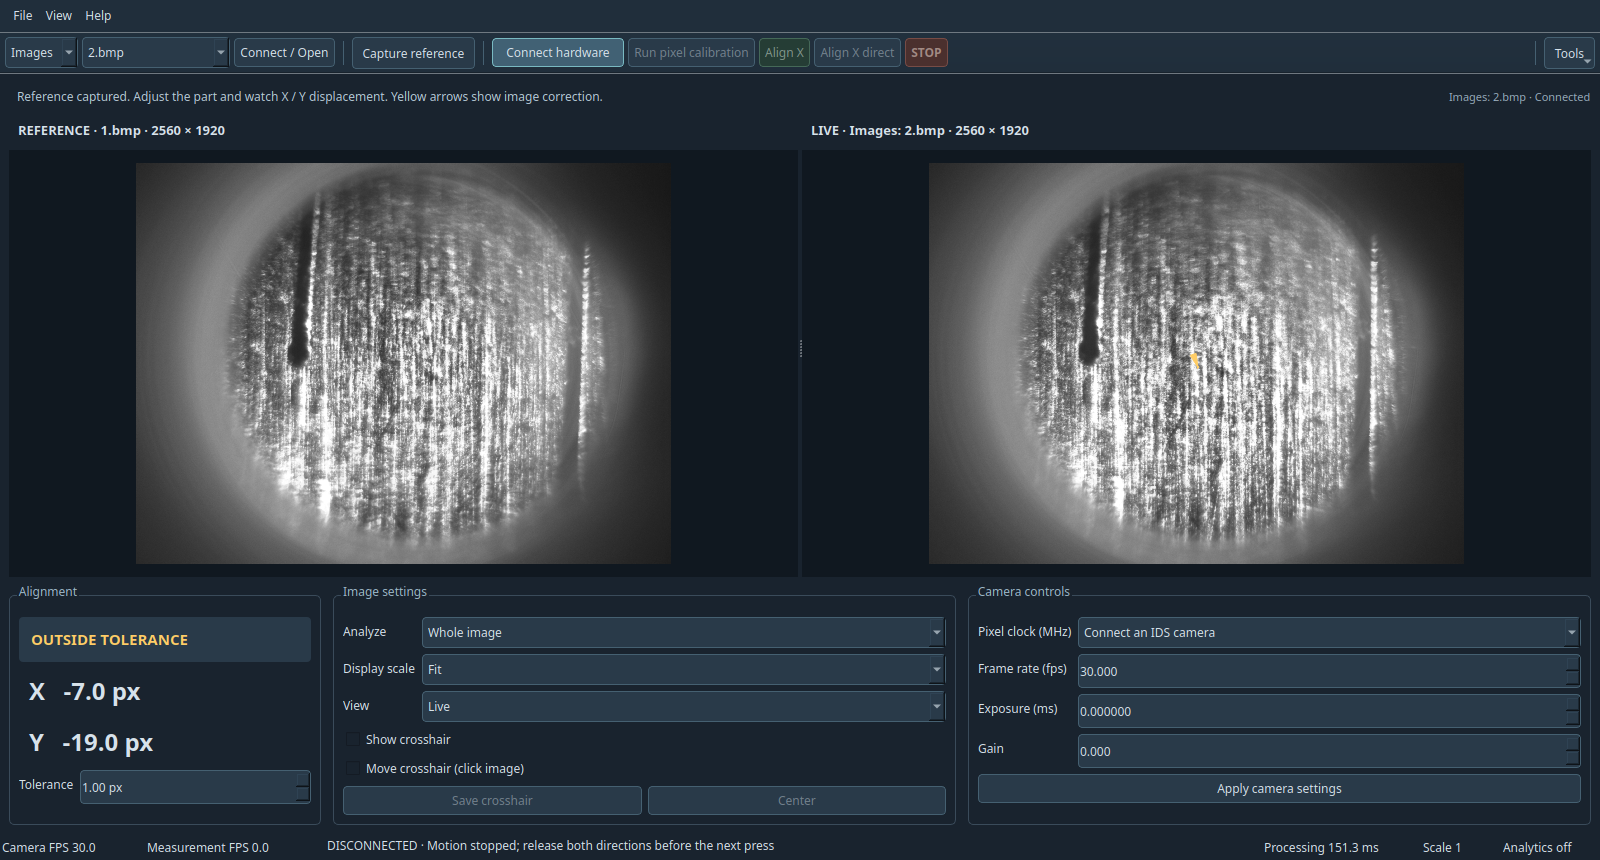
\includegraphics[width=0.90\linewidth]{assets/bedienoberflaeche.png}
  \par\smallskip
  {\small\textbf{Figure 1:} Screen overview using saved sample images.
  The operating procedure described here is performed using the joystick.}
\end{center}

\subsection{X and Y displacement}

The values indicate the displacement of the current image content relative
to the reference image in image pixels (px). X is horizontal; Y is vertical.

\begin{tabularx}{\linewidth}{@{}L{0.22\linewidth}Y@{}}
\toprule
\textbf{Reading} & \textbf{Meaning in the image} \\
\midrule
X positive / negative & Displaced to the right / left. \\
Y positive / negative & Displaced downwards / upwards. \\
\bottomrule
\end{tabularx}

The yellow arrow shows the required correction direction in the image.
Which joystick direction moves the image content to the left or right
depends on the configured setup. First observe the effect of a small movement.

\subsection{Assessing alignment}

\Note{X-axis correction.}{The motor axis corrects X only. Any remaining
Y displacement is not corrected by this joystick procedure. If Y is outside
the required tolerance, have the setup checked.}

The configured \textbf{Tolerance} applies to the combined distance in X and Y.
For example, with a tolerance of 1~px, X~=~0.8~px and Y~=~0.8~px together
are still outside tolerance. Use the status as the deciding indicator;
the numeric readout is slightly smoothed.

\Note{Software preview.}{Views labelled \textbf{Compensated} shift the image
in software only. A matching preview therefore does not confirm mechanical
alignment. Check the measured values and the actual overlap.}

\newpage
\section{Joystick operating instructions}

\subsection{Moving in steps}

Briefly move the joystick to the left or right, then release it. Each detected
directional input triggers one move using the configured step size. Holding
the joystick repeats the steps in sequence. After release, only the step
already in progress runs to completion.

Before changing direction, wait until the joystick is in its neutral position
and motion has stopped. Inputs released before the axis is ready are not
carried out later.

\subsection{Capturing a reference}

With the part stationary, press and release the \ReferenceButton{} once.
Holding the button does not capture additional images. Allow at least one
second between reference captures.

A new capture replaces the previous reference image. Check the position
before capturing. After restarting the application, capture the required
reference again using the joystick.

\subsection{Starting direct alignment}

Press and release the \AlignButton{} once, or click \textbf{Align X}.
The app compares the new X measurement after each relay nudge and chooses
the next direction from the change in error. Holding the button starts a
single attempt. Wait for the current operation to finish before pressing it again.

\subsection{Measuring displacement per press}

\textbf{Run pixel calibration} reports an optional measurement in pixels per
right press. In \textbf{Motion Setup}, set \textbf{Test presses} to a positive
number for right nudges or a negative number for left nudges. Keep the feature
visible throughout the test. The part stays at the final position.

\subsection{Cancelling an operation in progress}

To cancel calibration or automatic alignment in progress, briefly move the
joystick in either movement direction, then release it. The automatic
operation is cancelled. Wait until motion has stopped and the joystick is
in its neutral position before moving again or pressing the \AlignButton{}.
Releasing the align button alone does not cancel an operation in progress.

\newpage
\section{Status messages and troubleshooting}

The measurement display and the axis message describe different states.
Check both indicators if an operation is interrupted.

\begin{tabularx}{\linewidth}{@{}L{0.34\linewidth}Y@{}}
\toprule
\textbf{Display} & \textbf{Meaning and next step} \\
\midrule
\Status{ALIGNED} & The overall image displacement is within the configured tolerance. Check the image overlap. \\
\addlinespace
\Status{X aligned} & X is aligned. Also check Y and the overall status. \\
\addlinespace
\Status{OUTSIDE TOLERANCE} & The overall displacement is still too large. If X displacement remains, align again using the align button. Y is not corrected by the motor. \\
\addlinespace
\Status{NO REFERENCE} & The reference image is missing. Move to the reference position and press the reference button on the joystick. \\
\addlinespace
\Status{MATCH UNCERTAIN} & The image match is uncertain. Check the feature and overlap; if necessary, use the joystick to adjust the approximate position carefully. If the message persists, have the setup checked. \\
\addlinespace
\Status{PAUSED} & The image and measurements are not updating. The person responsible must restore live camera operation. \\
\addlinespace
\Status{DISCONNECTED} / \Status{STALE MEASUREMENT} & The connection or a current camera image is missing. Do not confirm alignment using these measurements. Have the connection and setup checked. \\
\bottomrule
\end{tabularx}

\subsection{A button does not respond}

Fully release the joystick and all buttons. Wait until the axis is stationary
and ready. Then press the required button again. A button pressed during
motion or before the axis is ready does not start an operation later. If the
button still does not respond, have the joystick assignments and connection
checked.

\subsection{Calibration or alignment does not finish}

Check that the same clearly identifiable feature remains in the image and
that the live image is up to date. After cancelling, return the joystick to
its neutral position and read the axis message. If the cause persists,
contact the person responsible for the setup. Do not press the
\ReferenceButton{} to eliminate an unwanted displacement; this would only
replace the reference image.

\smallskip
\textbf{Analytics:} Not required for this procedure. The analytics panel can
remain switched off; X/Y measurement continues.

\label{LastPage}
\end{document}
